\section{Background and Motivation}
\label{sec:overview}

\subsection{Identifier and Locator Separation}
%Since Saltzer's reflections on the distinction of names and addresses in networks~\cite{saltzer}, the idea of separating location and identity of network entities has attracted a plethora of incremental as well as clean-slate proposals for the design of future
%Internet. The main reason for this separation is its positive impact on four main requirements
%of a new Internet architecture as suggested in the Internet Research
%Task Force (IRTF) design goal document~\cite{li_design}: %These key
%requirements are
%routing scalability, mobility support, multi-homing support and traffic engineering enhancements.%, each of which has been
%shown to be addressable by the splitting of location and identity
%namespaces.

While there is broad agreement on identifier locator separation~\cite{saltzer,li},
implementation proposals vary widely along two main design
dimensions: (i) what does an identifier correspond to? and (ii) how is it
mapped to a locator? There are two main approaches.  In the
\emph{router-based} proposals such as LISP~\cite{farinacci},
Six/One~\cite{vogt-08} and APT~\cite{jen-apt-08}, the identifiers
identify
the network endpoints, and hosts can be reached by specifying the
endpoint through which they are connected to the network. Thus 
a host has to acquire a different endpoint identifier every time it
changes its network attachment point (though
patches to work around this problem have been
proposed~\cite{farinacci-mn}). In contrast, there is an alternative
\emph{host-based} approach in which identifiers are designated to
end hosts, resulting in each host maintaining its identifier
irrespective of changes in its point of attachment to the network.
%as shown in Figure~\ref{fig:router-host}.
HIP~\cite{moskowitz}, MILSA~\cite{milsa} and MobilityFirst~\cite{mobilityFirst} proposals have
shown the distinct benefits of having host-based identifiers in terms of
mobility support, multi-homing support and security, evidently at the
cost of requiring changes in the host-side protocol stack.

%Compared to this clear dichotomy in the meaning of identifiers, ideas about the
%other key implementation aspect, i.e., the
%Mapping schemes from identifiers to locator have mostly focused on the LISP approach~\cite{farinacci}. We, however, argue that requirements and assumptions in a host-based approach differ significantly from those of the router-based schemes and simple modifications of LISP based schemes are insufficient.
%do not lead to well
%performing solutions in this realm.

%    \begin{center}
%         %\vspace{-0.2in}
%         \begin{figure}[t!]
%             \centering
%             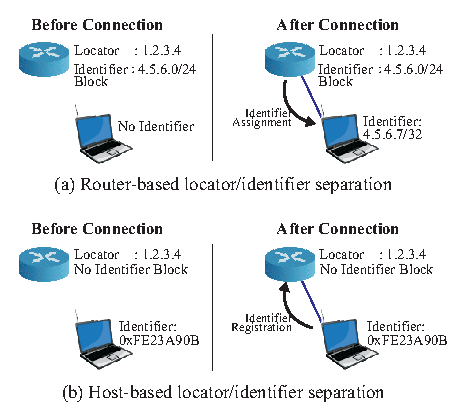
\includegraphics[width=0.4\textwidth]{figures/router-host.eps}             %\caption{Conceptual difference between router-based and
%               host-based separation schemes}
%             \label{fig:router-host}
%         \end{figure}
%     \vspace{-0.3in}
%     \end{center}

 \subsection{Requirements of Host-Based Identifiers}

We believe that a host-based mapping scheme must meet the following
requirements:

 \begin{itemize}
 	\item
  {\bf Flat Identifiers:} The mapping architecture needs to support
  structure-less, flat identifiers. %which is a central dogma of
  %HIP and MobilityFirst. %LISP-ALT~\cite{farinacci-alt},
  %LISP-DHT~\cite{mathy}, SLIMS~\cite{hou-09} and other LISP based
  %mapping schemes make use of aggregation in the identifier namespace
  %and they do not scale without that assumption.

 	\item
 {\bf Low Latency:} Since mobility is directly handled using dynamic
 identifier to locator mapping, latency requirements are much stricter
 in host-based schemes. %In particular, the MobilityFirst proposal
 %includes support for identifier-locator querying by network routers
 %for in-transit packets which could result in multiple mapping queries
 %during the transmission of a single packet. Thus low latency is a
 %fundamental requirement. %{\bf [How fast is enough for routing? How
 %    much mobile routing can be improved by our scheme]}

 	\item
 {\bf Low Staleness:} Fast mobility support also requires that the
 identifier-locator mappings be updated at a time-scale smaller than
 the inter-query time.% produced from anticipated mobility patterns. %Thus
 %traditional DNS based schemes, despite its low query latencies are not
 %suitable.{\bf [Prove that DNS doesn\'t satisfy fast mobility
 %    requirement, even with ]}

 	\item
 {\bf Storage Scalability:} Since flat identifiers would lead to
 substantially more number of identifier to locator entries, the
 mapping scheme needs to scale to the order of billions of entries
 instead of thousands~\cite{cisco-2010}.
 \end{itemize}

% Due to their inherent design trade-offs, the traditional approaches
% for such kind of mapping storage do not fare well in terms of one or
% more of the above mentioned requirements. In particular, BGP based
% announcement schemes rely on aggregation of identifiers for
% propagation of mapping data, DNS based schemes rely on extensive
% caching which cannot support large scale mobility and DHT based
% schemes that have the desirable quality of distributed storage result
% in either substantially higher query latencies or prohibitive table
% maintenance overhead.




 %Given the number of identifier-locator mapping schemes recently
 % proposed, the natural place to start is by exploring

The above requirements call for a fundamental shift from traditional
mechanisms such as MobileIP, DNS and DHT.
While it is applicable at small scale, the mapping scheme of MobileIP
incurs high overhead since all mappings are resolved by the home agent
regardless of its distance to correspondents. A home agent acting as a
relaying node on the data plane in tunnelling mode makes MobileIP not
scalable to global Internet scale. On the other hand, since it relies
on extensive caching, DNS cannot deal with fast updates. In addition,
to store the mappings of billions of hosts and handle their
updates/queries, a much larger dedicated infrastructure than
the current DNS would be required. Traditional Distributed Hash
Table (DHT) schemes and their optimized variations, e.g., \cite{monnerat,
  gupta}, aim to solve the problems of centralized solutions but
invariably introduce a fundamental tradeoff between service latency
and table/maintenance overhead.
  A detailed discussion of other existing mechanisms along with their pros and cons are presented in Section \ref{sec:related}.   
  %As Carpenter succinctly
 %identified~\cite{carpenter}, the design of any mapping scheme which
 %enables location/identifier separation in the future Internet depends
 %on the implicit or explicit assumptions made on certain key factors
 %answering the following questions: - Should the scheme depend on the
 %identifier space? What is the expected scale of identifier namespaces?
 %Is the mapping invoked only upon the start of transmission or at
 %successive domain boundaries while a packet is in-transit? What is the
 %lifetime of a mapping? Should the scheme support dynamic
 %identifier-locator mapping for mobility? and Does the mapping scheme
 % have any impact on privacy? The design choices made by most of the
 %existing proposals focus on a subset of these issues while giving less
 %priority to other key requirements, especially those which directly
 %affect mobility support. As a concrete example, the MobilityFirst
 %proposal includes support for identifier-locator querying by network
 %routers for in-transit packets which could result in multiple mapping
 %queries on course the transmission of a single packet. Clearly, in
 %this use-case, LISP-TREE with an average latency of around half a
 %second or LISP-DHT with query times going up to a second cannot be
 %readily used. The ABCD approach is motivated by the limitations of the
 %two basic mechanisms for directory lookup type service, i.e., the DHT
 %based schemes and the DNS based schemes.
 %
 %% {\bf The need of a new fast and scalable mapping scheme}
%% %% handoffs:  802.21  UMA (unlicensed mobile access) , 3GPPP
%% %% (Wifi/GSM) GAN (generic access network)
%
%% The XYZ design is motivated by two key insights:
%
% \begin{itemize}
% \item \emph{MobileIP}. The mapping scheme of MobileIP incurs high overhead, low
%   scalability, and a single point of failure. All mappings are resolved
%   by the home agent regardless of its distance to correspondents. The home
%  agent must act as a relaying node on the data plane in tunneling mode.
%
%
%\item \emph{DNS}. Centralized overlay resolution services similar to DNS that
%   rely on extensive caching cannot deal with fast updates. In
%   addition, to store the mappings of billions of hosts and handle
%   their updates/queries,  a much larger dedicated infrastructure support
%   than the current DNS would be required.
%
% \item \emph{Distribute Hash Table (DHT)}. Traditional DHT schemes such as Chord~\cite{stoica}, CAN~\cite{ratnasamy}, etc. as well as their optimized variations
%  such as those described in~\cite{monnerat, gupta}, etc. aim to solve
%   the problems of centralized solutions but invariably introduce a
%   fundamental tradeoff between service latency and
%   table/maintenance overhead.
%
% \end{itemize}



%%To address these problems, in this work, we propose a mapping mechanism, \emph{Direct Mapping (DMap)} built on the  principle of shared hosting of the locator/identifier mappings
%%among all the ASs in the network. While our solution
 %targets the aforementioned dearth of host-based identifier to locator
 %mapping schemes and can be utilized for implementing any of the
 %host-based proposals, in this paper we focus on its application to the
 %MobilityFirst architecture.
% DMap highlights a key difference
% between the router-based and the host-based schemes: the identifiers
% in the router-based scheme, being used to identify network endpoints,
% are \emph{owned} by networks and thus the mappings of the set of identifiers owned by an AS are stored and
% managed by that AS. In contrast, each identifier in the host-based
% scheme denotes a host which \emph{happens to be connected} to a
% particular AS. With increasing trends of mobile hosts which often also
% have multiple simultaneous points of network attachment, the concept of `owner' of a particular identifier
% thus becomes fuzzy. Even though traditionally, the AS primarily
% serving a host becomes its de facto owner and manages its mappings, we
% challenge this assumed constraint in the favor of a network-wide
% sharing of the identifier-locator mappings independent of the AS
% boundaries.


 %Under this conceptual shift from ASs `owning' endpoint identifiers and
 %individually storing the mappings of its owned set of identifiers to a
 %seamless sharing of the mappings across AS boundaries, the identifier
 %to locator mapping for an identifier $X$ in AS $A$ will be stored in a
 %set of foreign ASs $\{B_1, B_2, \ldots, B_k\}$ instead of being stored
 %in $A$ itself. The key advantage of this shared hosting is that we
 %can make $B_is$ as being deterministically derived from $X$ and
 %leverage the routing infrastructure to reach $B_is$ in a single
 %overlay hop. In particular, we define a direct hashing scheme which
 %hashes the value of $X$ to a set of $k$ routable addresses and chooses
 %the $B_i$ that advertises each of these addresses in the global
 %routing protocol. This leads to drastically reduced mapping resolution
 %latency compared to DHT based schemes without requiring any DNS like
 %infrastructure services.

 %The aim of this paper is to evaluate the feasibility of such a scheme,
 %compare its latency and scalability with previously defined mechanisms
 %and also to address the evident concern about incentive -

\subsection{Incentive for Shared Hosting}

To address the problems above, in this work, we propose DMap which is
built on the principle of shared hosting of the locator to identifier
mappings among all the ASs in the network.  A concern that may arise
naturally with shared hosting is incentive: \emph{why
  would Network Operator A store and manage Network Operator B's
  identifiers?} As we argued above, with host-based identifiers, the
concept of site-dependent or provider-dependent identifiers are
diluted specially in the case of mobile hosts. For fixed legacy hosts,
we assert that just like peer-to-peer file sharing systems and TCP
congestion control, cooperative schemes that result in a common good
with a small individual cost have a natural incentive mechanism for
deployment as long as the individual cost of participation is
reasonable. In particular, the incentives for foul-play, i.e., not
storing or answering mapping requests in this case, would depend on
the benefit vs. possible penalty of non-compliance. Both technical
solutions (such as reputation management in peer-to-peer systems) and
non-technical policy bindings (analogous to Network Neutrality
arguments) can be invoked to force/persuade ASs to fairly participate
in the scheme. However, in this paper, we focus on the architectural
and performance aspects of the scheme and leave the design of the
incentive mechanisms open.
 %As we show through simulation based evaluation, our scheme
 %results in `proportional fairness' of mapping assignments, in the
 %sense that as AS which is expected to generate a large number of
 %identifier to locator mapping requests from other ASs, itself will
 %have to store and answer a proportionally large number of
 %mappings. While we address the incentive and privacy issues raised by
 %this ideological shift, our main goal here is to challenge the
 %presumed constraint of fixed, ownership based mechanisms and explore
 %if a more efficient co-operative scheme is feasible.

%% In order to gain more insights into the requirements of the envisioned
%% mapping scheme and highlight the difference in its usage compared to
%% similar schemes for the LISP proposal, we provide a brief overview of
%% the MobilityFirst architecture, enabling which is a key focus of the
%% XYZ scheme.

%% MobilityFirst is a `clean-slate' future Internet architecture project
%% funded by the NSF FIA program~\cite{fia} with a particular focus on
%% supporting large-scale, efficient and robust mobility services in the
%% future Internet. The architecture is motivated by the dramatic growth
%% of mobile devices and applications on the Internet and targets the
%% projected dominance of mobile Internet traffic over that of fixed
%% hosts in the near future~\cite{cisco-2010}. As depicted in
%% Figure~\ref{fig:mobilityFirst} (reproduced from~\cite{nelson-11}), a
%% central principle of the architecture is that every host has a
%% permanent, location independent, globally unique identifier (GUID)
%% which can then be mapped to a set of routable locators or network
%% addresses (NA) corresponding to the current point(s) of attachment. In
%% addition to hosts, GUIDs can refer to content and context to provide
%% seamless content and context handling support in the future
%% Internet. In terms of mapping scheme requirements, this leads to a
%% much larger number of identifiers than the projected number of hosts
%% usually considered in LISP based schemes. The MobilityFirst proposal
%% includes late or repeated binding support, i.e., resolving a GUID to a
%% network address at different points along the route in order to
%% support rapid host mobility. This creates stricter latency
%% requirements for the mapping lookups. Another aspect of the design
%% which affects the mapping scheme is storage aware routing which gives
%% routers the option to temporarily store data as a network-layer
%% routing decision. Retransmitting the stored packets would require
%% another mapping lookup leading to a much higher number of lookups
%% compared to LISP based
